\documentclass[12pt]{article}
% Load packages
\usepackage{url}  % Formatting web addresses
\usepackage{ifthen}  % Conditional
\usepackage{multicol}   %Columns
\usepackage[utf8]{inputenc} %unicode support
\usepackage{amsmath}
\usepackage{amssymb}
\usepackage{mathtools}
\usepackage{epsfig}
\usepackage{epstopdf}
\usepackage{graphicx}
\usepackage[margin=0.1pt,font=footnotesize,labelfont=bf]{caption}
\usepackage{setspace}
%\usepackage{longtable}
\usepackage{colortbl}
%\usepackage{palatino,lettrine}
%\usepackage{times}
%\usepackage[applemac]{inputenc} %applemac support if unicode package fails
%\usepackage[latin1]{inputenc} %UNIX support if unicode package fails
\usepackage[wide]{sidecap}
%\usepackage[authoryear,round,comma,sort&compress]{natbib}
\usepackage[square,sort,comma,numbers,sort&compress]{natbib}
%\usepackage[authoryear,round]{natbib}
\usepackage{supertabular}
\usepackage{simplemargins}
\usepackage{fullpage}
\usepackage{comment}
\usepackage{lineno}
%\usepackage{chicago}
\usepackage{textcomp}
\usepackage{multirow}
\usepackage{amsmath}
\usepackage[linesnumbered,lined,boxed,commentsnumbered]{algorithm2e}
\DeclareMathOperator*{\argmin}{\arg\!\min}

\usepackage{algorithm2e}
\usepackage{algpseudocode}
%\usepackage[space]{cite}
\urlstyle{rm}

%\textwidth = 6.50 in
%\textheight = 9.5 in
%\oddsidemargin =  0.0 in
%\evensidemargin = 0.0 in
%\topmargin = -0.50 in
%\headheight = 0.0 in
%\headsep = 0.25 in
%\parskip = 0.15in
%\linespread{1.75}
\doublespace

%\bibliographystyle{chicago}
\bibliographystyle{plos2009}

\makeatletter
\renewcommand\subsection{\@startsection
	{subsection}{2}{0mm}
	{-0.05in}
	{-0.5\baselineskip}
	{\normalfont\normalsize\bfseries}}
\renewcommand\subsubsection{\@startsection
	{subsubsection}{2}{0mm}
	{-0.05in}
	{-0.5\baselineskip}
	{\normalfont\normalsize\itshape}}
\renewcommand\section{\@startsection
	{subsection}{2}{0mm}
	{-0.2in}
	{0.05\baselineskip}
	{\normalfont\large\bfseries}}
\renewcommand\paragraph{\@startsection
	{paragraph}{2}{0mm}
	{-0.05in}
	{-0.5\baselineskip}
	{\normalfont\normalsize\itshape}}
\makeatother

%Review style settings
%\newenvironment{bmcformat}{\begin{raggedright}\baselineskip20pt\sloppy\setboolean{publ}{false}}{\end{raggedright}\baselineskip20pt\sloppy}

%Publication style settings

% Single space'd bib -
\setlength\bibsep{0pt}

\renewcommand{\rmdefault}{phv}\renewcommand{\sfdefault}{phv}
\newcommand{\norm}[1]{\left\lVert#1\right\rVert}

% Change the number format in the ref list -
\renewcommand{\bibnumfmt}[1]{#1.}

% Change Figure to Fig.
\renewcommand{\figurename}{Fig.}

% Begin ...
\begin{document}
\begin{titlepage}
{\par\centering\textbf{\Large {Analysis of TX-TL Synthetic Circuits using Sequence Specific Constraints Based Modeling}}}
\vspace{0.05in}
{\par \centering \large{Jeffrey D. Varner$^{*}$}}
\vspace{0.10in}
{\par \centering {School of Chemical and Biomolecular Engineering}}
{\par \centering {Cornell University, Ithaca NY 14853}}
\vspace{0.1in}
{\par \centering \textbf{Running Title:}~Constraints based models of synthetic circuits}
\vspace{0.1in}
{\par \centering \textbf{To be submitted:}~\emph{Scientific~Reports}}
\vspace{0.5in}
{\par \centering $^{*}$Corresponding author:}
{\par \centering Jeffrey D. Varner,}
{\par \centering Professor, School of Chemical and Biomolecular Engineering,}
{\par \centering 244 Olin Hall, Cornell University, Ithaca NY, 14853}
{\par \centering Email: jdv27@cornell.edu}
{\par \centering Phone: (607) 255 - 4258}
{\par \centering Fax: (607) 255 - 9166}
\end{titlepage}
\date{}
\thispagestyle{empty}
\pagebreak
%%%%%%%%%%%%%%%%%%%%%%%%%%%%%%%%%%%%%%%%%%%%%%%%%%%%%%%%%%%%%%%%%%%%%%%%%%%%%%%%%%%%%%%%%%%%%%%%%%%%%%%%%%%
%%%%%%%%%%%%%%%%%%%%%%%%%%%%%%%%%%%%%%%%%%%%%%%%%%%%%%%%%%%%%%%%%%%%%%%%%%%%%%%%%%%%%%%%%%%%%%%%%%%%%%%%%%%
\section*{Abstract}

In this study, we used sequence specific constraints based modeling to evaluate the performance of synthetic circuits in an \emph{E.~coli} TX-TL system.
A core \emph{E.~coli} metabolic model, consisting of XX metabolites and YY reactions, was developed from literature [REF].
This model, which described glycolysis, pentose phosphate pathway, amino acid biosynthesis and degradation and energy metabolism, was then augmented with
sequence specific descriptions of genetic circuits which included mechanistic models of promoter function, transcription and translation.
Thus, unlike other synthetic biology modeling efforts, sequence specific constraints based modeling explicitly couples
the transcription and translation of circuit components with the availability of metabolic resources.
Model parameters were largely taken from literature; our approach had very few adjustable parameters thereby allowing the a first principles prediction of circuit performance.
We tested this approach by first simulating $\sigma_{70}$-induced deGFP expression and then expanded these studies to more complex multicomponent circuits.
First principles predictions of circuit performance were consistent with measurements for a variety of cases.
Further, global sensitivity analysis identified the key metabolic processes that controlled circuit performance.
Taken together, sequence specific constraints based modeling offers a novel means to \emph{a~priori} estimate the performance of cell free synthetic circuits.

\vspace{0.1in}
{\noindent \textbf{Keywords:}~Synthetic biology, Constraints based modeling, Biochemical modeling}


\pagebreak

\setcounter{page}{1}

\linenumbers


\section*{Introduction}

Cell free systems offer many advantages for the study, manipulation and modeling of metabolism compared to \textit{in vivo} processes.
Central amongst these advantages is direct access to metabolites and the microbial biosynthetic machinery without the interference of a cell wall.
This allows us to control as well as interrogate the chemical environment while the biosynthetic machinery is operating, potentially at a fine time resolution.
Second, cell-free systems also allow us to study biological processes without the complications associated with cell growth.
Cell-free protein synthesis (CFPS) systems are arguably the most prominent examples of cell-free systems used today \citep{Jewett:2008aa}.
However, CFPS is not new; CFPS in crude \textit{E. coli} extracts has been used since the 1960s to explore fundamentally important biological mechanisms \citep{MATTHAEI:1961aa,NIRENBERG:1961aa}.
Today, cell-free systems are used in a variety of applications ranging from therapeutic protein production \citep{Lu:2014aa} to synthetic biology \citep{Hodgman:2012aa}.
Interestingly, many of the challenges confronting in-vivo genome-scale kinetic modeling can potentially be overcome in a cell-free system.
For example, there is no complex transcriptional regulation to consider, transient metabolic measurements are easier to obtain, and we no longer have to consider cell growth.
Thus, cell-free operation holds several significant advantages for model development, identification and validation.
Theoretically, genome-scale cell-free kinetic models may be possible for industrially important organisms, such as \textit{E. coli} or \textit{B. subtilis}, if a simple, tractable framework for integrating allosteric regulation with enzyme kinetics can be formulated.

Stoichiometric reconstructions of microbial metabolism popularized by constraint based modeling techniques such as flux balance analysis (FBA) have become standard tools to interrogate biological networks \citep{2012_lewis_palsson_NatRevMicrobio}.
Since the first genome-scale stoichiometric model of \textit{E. coli}, developed by Edwards and Palsson \citep{2000_edwards_palsson_PNAS}, stoichiometric reconstructions of hundreds of organisms, including industrially important prokaryotes such as \textit{E. coli} \citep{Feist:2007aa} or \textit{B. subtilis} \citep{Oh:2007aa}, are now available \citep{2009_feist_palsson_NatRevMicrobio}.
Stoichiometric models rely on a pseudo-steady-state assumption to reduce unidentifiable genome-scale kinetic models to an underdetermined linear algebraic system, which can be solved efficiently even for large systems using linear programming.
Traditionally, stoichiometric models have also neglected explicit descriptions of metabolic regulation and control mechanisms, instead opting to describe the choice of pathways by prescribing an objective function on metabolism.
Interestingly, similar to early cybernetic models, the most common metabolic objective function has been the optimization of biomass formation \citep{2002_ibarra_edwards_palsson_Nat}, although other metabolic objectives have also been estimated \citep{2007_schuetz_sauer_MolSysBio}.
Recent advances in constraint-based modeling have overcome the early shortcomings of the platform, including capturing metabolic regulation and control \citep{2013_hyduke_lewis_palsson_MolBioSys}. Thus, modern constraint-based approaches are extremely useful for the discovery of metabolic engineering strategies and represent the state of the art in metabolic modeling \citep{2013_mccloskey_palsson_feist_MolSysBio, 2012_zomorrodi_maranas_MetaEng}.

In this study, we used sequence specific constraints based modeling to evaluate the performance of synthetic circuits in an \emph{E.~coli} TX-TL system.
A core \emph{E.~coli} cell free metabolic model, consisting of XX metabolites and YY reactions, was developed from literature [REF].
This model, which described glycolysis, pentose phosphate pathway, amino acid biosynthesis and degradation and energy metabolism, was then augmented with
sequence specific descriptions of genetic circuits which included mechanistic models of promoter function, transcription and translation.
Thus, sequence specific constraints based modeling explicitly couples
the transcription and translation of circuit components with the availability of metabolic resources.
Model parameters were largely taken from literature; our approach had very few adjustable parameters thereby allowing the a first principles prediction of circuit performance.
We tested this approach by first simulating $\sigma_{70}$-induced deGFP expression and then expanded these studies to more complex multicomponent circuits.
First principles predictions of circuit performance were consistent with measurements for a variety of cases.
Further, global sensitivity analysis identified the key metabolic processes that controlled circuit performance.
Taken together, sequence specific constraints based modeling offers a novel means to \emph{a~priori} estimate the performance of cell free synthetic circuits.

\clearpage

%Constraints based models are important tools to understand and ultimately to predict how cells utilize nutrients to produce products.
%Constraints based methods such as flux balance analysis (FBA) \cite{2010_orth_NatBiotech} and network decomposition approaches such as elementary modes (EMs) \cite{Schuster:2000aa}
%or extreme pathways (EPs) \cite{Schilling:2000aa}
%model intracellular metabolism using the biochemical stoichiometry and other constraints such as thermodynamical feasibility under pseudo-steady state conditions.
%FBA has been used to efficiently estimate the performance of metabolic networks of arbitrary complexity, including genome scale networks, using linear programming  \cite{Covert:2004aa}.
%On the other hand, EMs (or EPs) catalog all possible metabolic behaviors such that any flux distribution predicted by FBA is a convex combination
%of the EMs (or EPs) \cite{Wiback:2003aa}.
%However, the calculation of EMs (or EPs) is computationally expensive and currently infeasible for genome scale networks \cite{2004_lee_varner_ko_ieee}.



\section*{Results}
The protein concentration levels of deGFP produced with TX-TL 2.0 at different plasmid concentrations was modeled using a sequence specific constraints based modeling approach in a \textit{E. coli} cell free network (Fig. \ref{fig:deGFP_Plasmid}).
The metabolic network was formulated by removing all cell wall associated reactions and incorporating amino acid synthesis and transcription/translation associated reactions. 
The network consisted of 281 reactions and 132 species. 
The transcription and translation rates were constrained to experimental measurements \cite{2016_Garamella_etal_TXTL} for the RNA polymerase and ribosome elongation rates. 
The production time for TX-TL 2.0 is approximately 8 hours \cite{2016_Garamella_etal_TXTL}. 
The concentration of deGFP was determined at each plasmid concentration by multiplying the corresponding production flux by the production time. 
The sequence specific constraints based model was able to capture the deGFP concentration up to a plasmid concentration of 5 nM and overestimates deGFP measurements above that.
TX-TL 2.0 has a saturation on protein production mostly due to limited resources which our model begins to see saturating effects at ~9 nM plasmid concentration. 
This may be due to oxidative phosphorylation activity which has been observed to take place in other cell free systems \cite{2008_Jewett_etal_OxPhos}.

\begin{figure}[!t]\centering
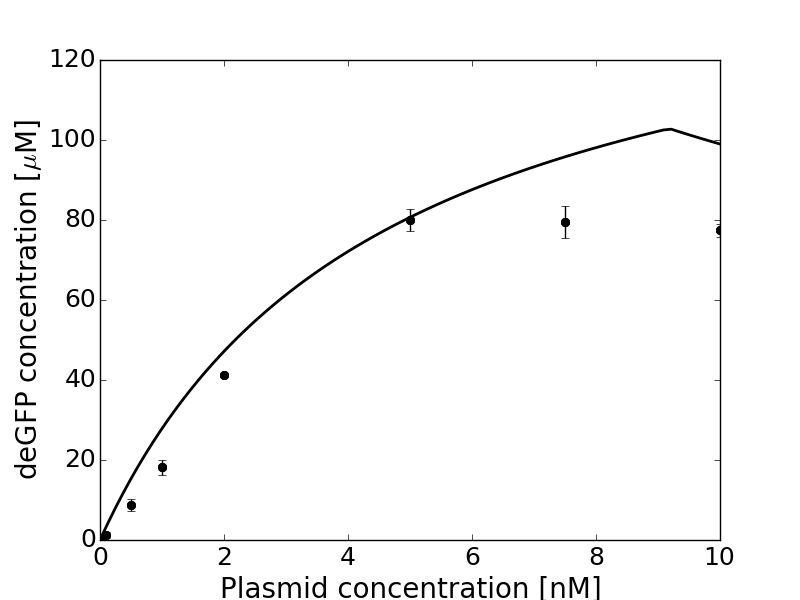
\includegraphics[width=0.45\textwidth]{./figures/deGFP_Plasmid.png}
\caption{Model simulation (solid line) versus deGFP protein concentration (dots) at different plasmid concentrations produced in TX-TL 2.0. 
}
\label{fig:deGFP_Plasmid}
\end{figure}

\begin{figure}[!t]\centering
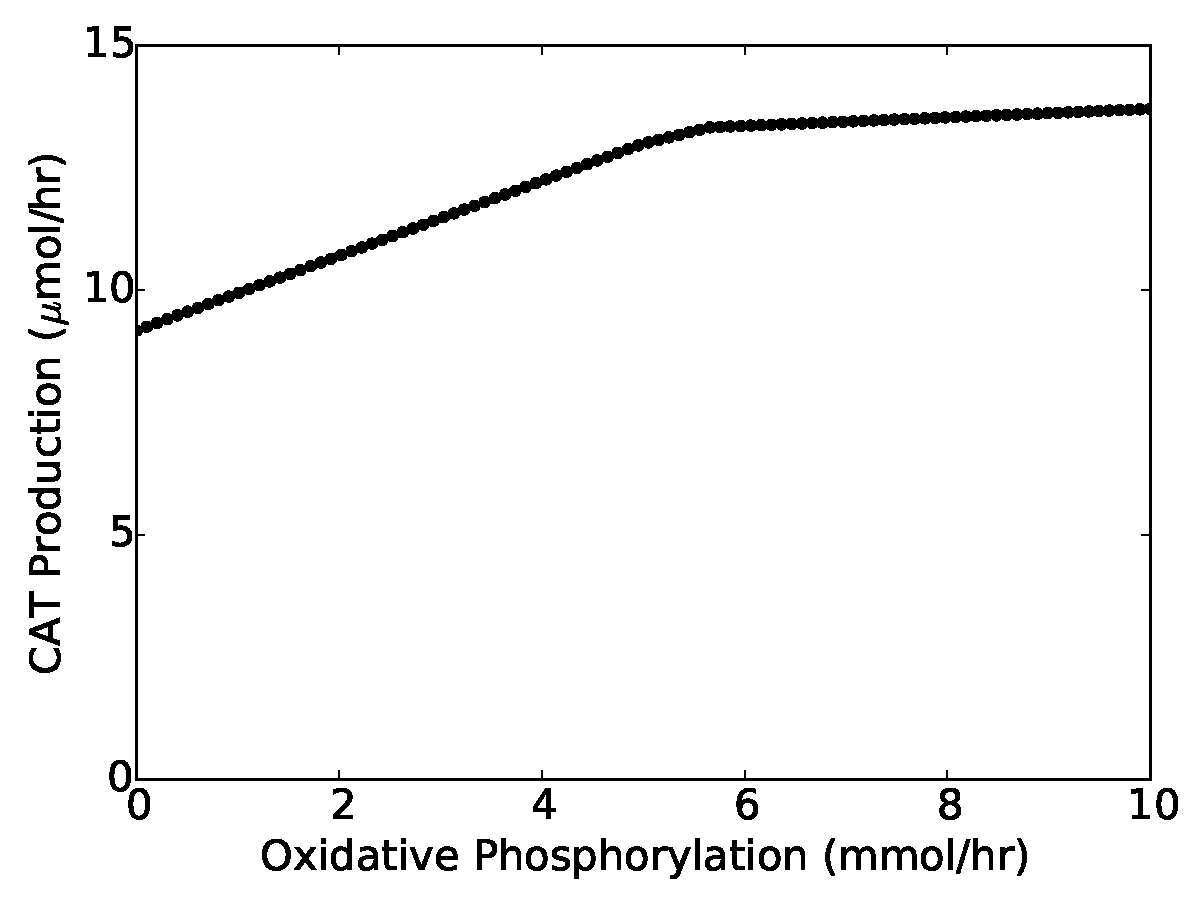
\includegraphics[width=0.45\textwidth]{./figures/CAT_oxphos.pdf}
\caption{
}
\label{fig:CAT_oxphos}
\end{figure}

Oxidative phosphorylation activity influences the protein production flux as well as acetate and lactate flux.    
Our model suggests higher oxidative phosphorylation activity increases the protein production rate for CAT (Fig. \ref{fig:oxphos.pdf}) and other proteins. 
Consistent with literature, limiting oxidative phosphorylation results in lower protein yields in cell free systems as seen in our model. 
Oxidative phosphorylation activity was limited to have a maximum flux of 3.0 mmol/hr in it's reactions, determined from a tradeoff between acetate and lactate flux (Fig. \ref{fig:oxhos}). 
Experimental data has shown lactate and acetate to have similar fluxes during glucose consumption during the production of CAT (data not shown).
Low oxidative phosphorylation leads to NADH overflow which is re-oxidized with lactate dehydrogenase reducing pyruvate to lactate leading to high lactate formation.
High oxidative phosphorylation relative to our cell free system leads to lower lactate and higher acetate formation.

%\begin{figure}[!t]\centering
%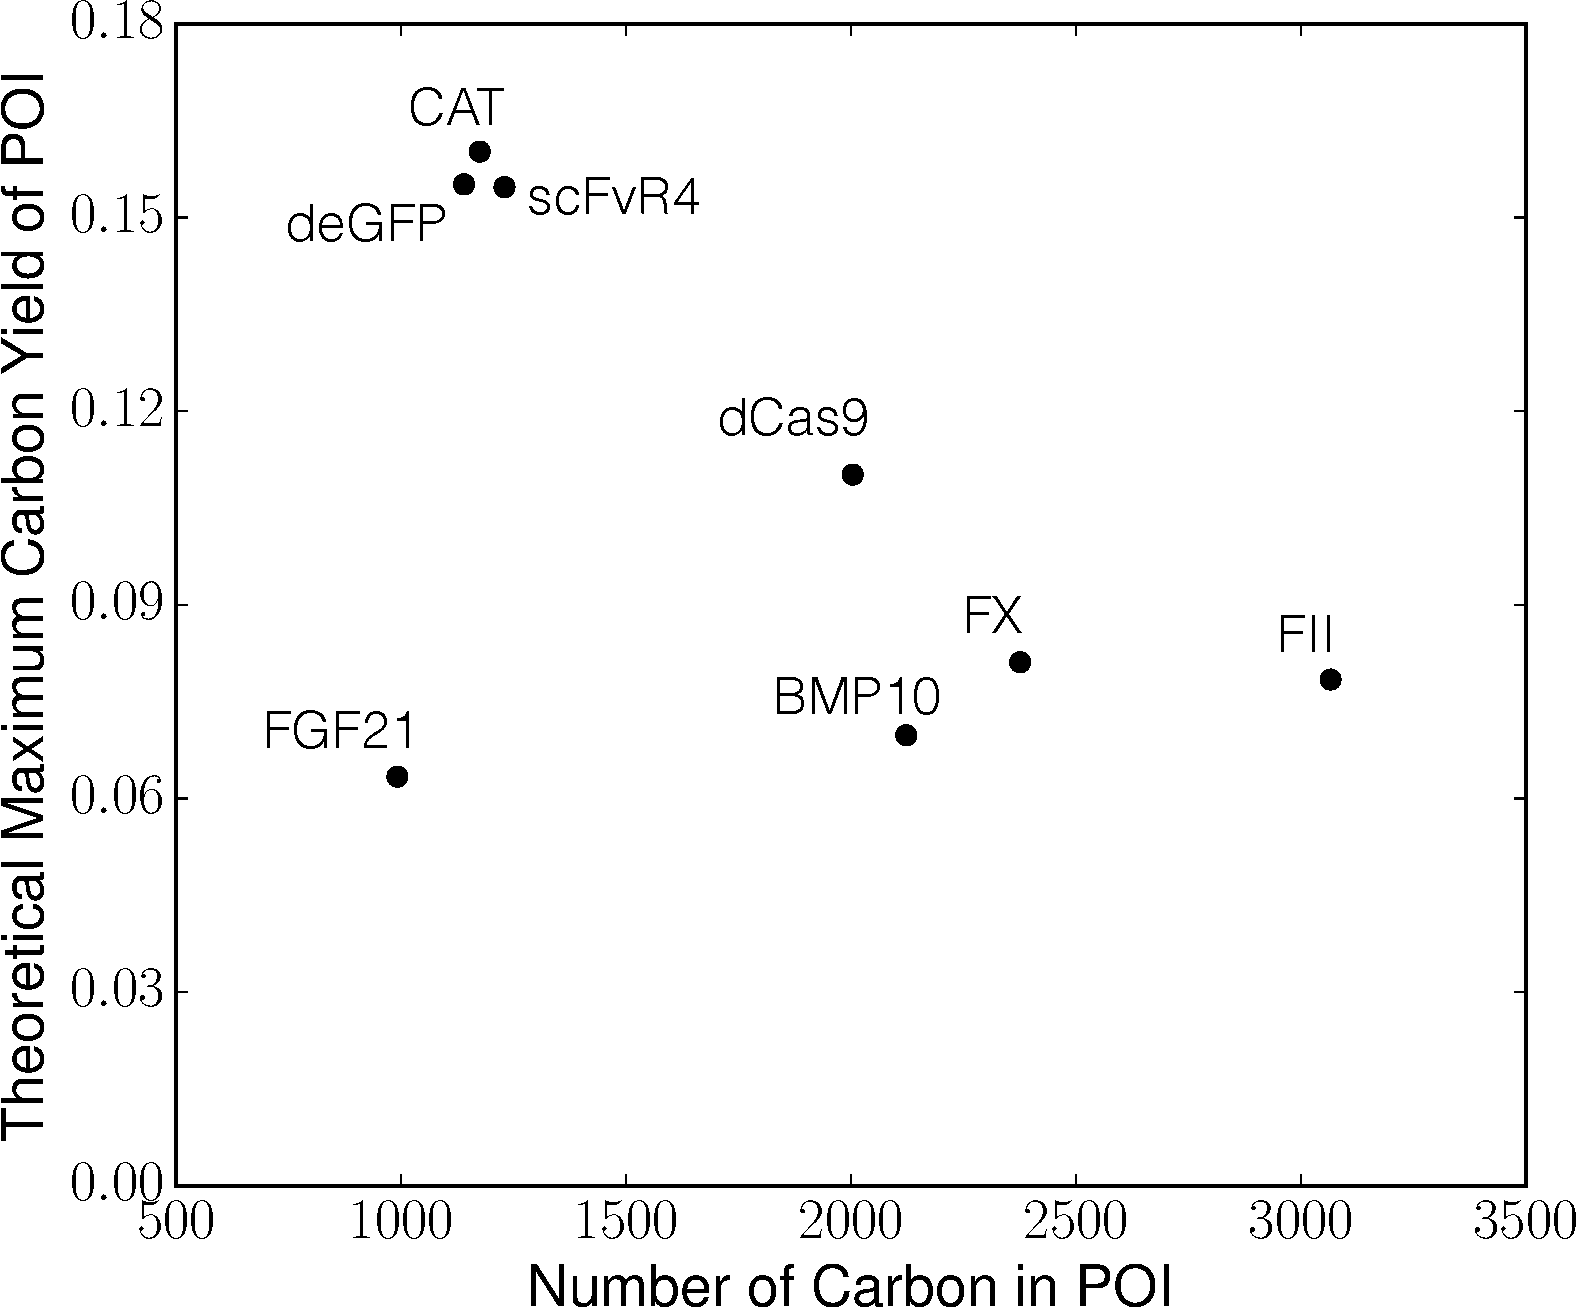
\includegraphics[width=0.45\textwidth]{./figures/YieldNumber.pdf}
%\caption{Oxidative phosphorylation activity influences protein, acetate and lactate production. A) Increasing oxidative phosphorylation leads to higher protein (CAT) production %rates and begins to saturate. B) Lactate versus acetate flux at different oxidative phosphorylation activity levels. As oxidative phosphorylation increases, lactate formation %decreases and acetate formation increases.
%}
%\label{fig:oxphos}
%\end{figure}

Theoritical carbon yields were calculated for nine different proteins using a sequence specific constraints based modeling approach in a \textit{E. coli} cell free network. 
Carbon yields were calculated for three different cases: unconstrained, limited oxidative phosphorylation and TX-TL constraints (Fig. \ref{fig:CarbonYield}). 
In the unconstrained case, amino acids uptake and oxidative phosphorylation activity were unbounded. 
Most of the proteins studied in this paper resulted in a carbon yield near forty percent for a cell free system.
In the limited oxidative phosphorylation case, carbon yields were reduced for each of the proteins. 
   
In the TX-TL 2.0 case, oxidative phosphorylation activity was limited in addition to limited transcription and translation fluxes.
Following these constraints, an optimal plasmid concentration was determined for each protein which was used to determine the carbon yield for TX-TL 2.0 at that plasmid concentration.
Carbon yields are significantly reduced compared to the unconstrained and limited oxidative phosphorylation cases.
The carbon yields are being lost mostly due to lactate and acetate formation.
The constrained TX-TL case requires additional ATP to optimize for the protein of interest production leading to acetate formation.

TX-TL 2.0 carbon yields were then compared to the carbon number of each protein of interest (Fig. \ref{fig:YieldNumber}). 
There is a relative inverse relationship between the carbon yield and the carbon number of each protein with the exception of FGF21. 
In comparing the amino acids of each protein, the proteins with a carbon yield below ten percent have a high abundance of proline which is a non polar amino acid and may have a negative impact on increasing carbon yield. 

\begin{figure*}[!t]\centering
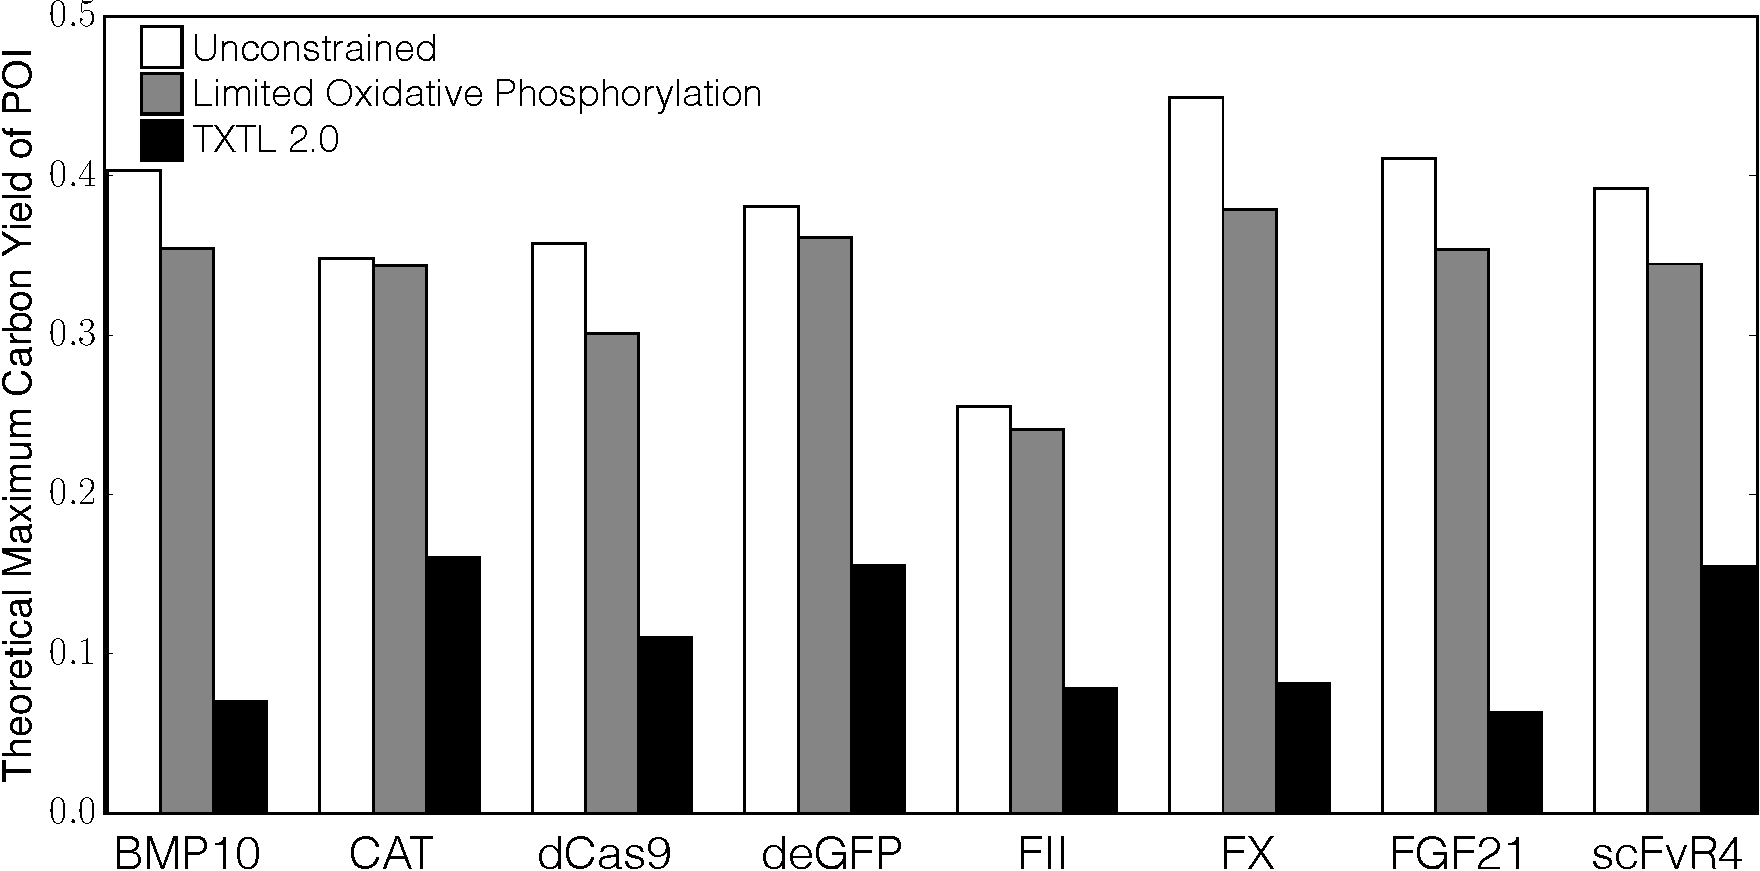
\includegraphics[width=0.90\textwidth]{./figures/CarbonYield.pdf}
\caption{Theoriticcal carbon yield of nine different proteins for three different cases in a cell free system. 
Unconstrained yields (white bar) produced the highest carbon yield out of the three cases. In the limited oxidative phosphorylation case (gray bar), carbon yields were slightly lower than for the unconstrained case. TXTL 2.0 (black bar) constraints had low carbon yields compared to unconstrained and limited oxidative phosphorylation cases. 
}
\label{fig:CarbonYield}
\end{figure*}

\begin{figure}[!t]\centering
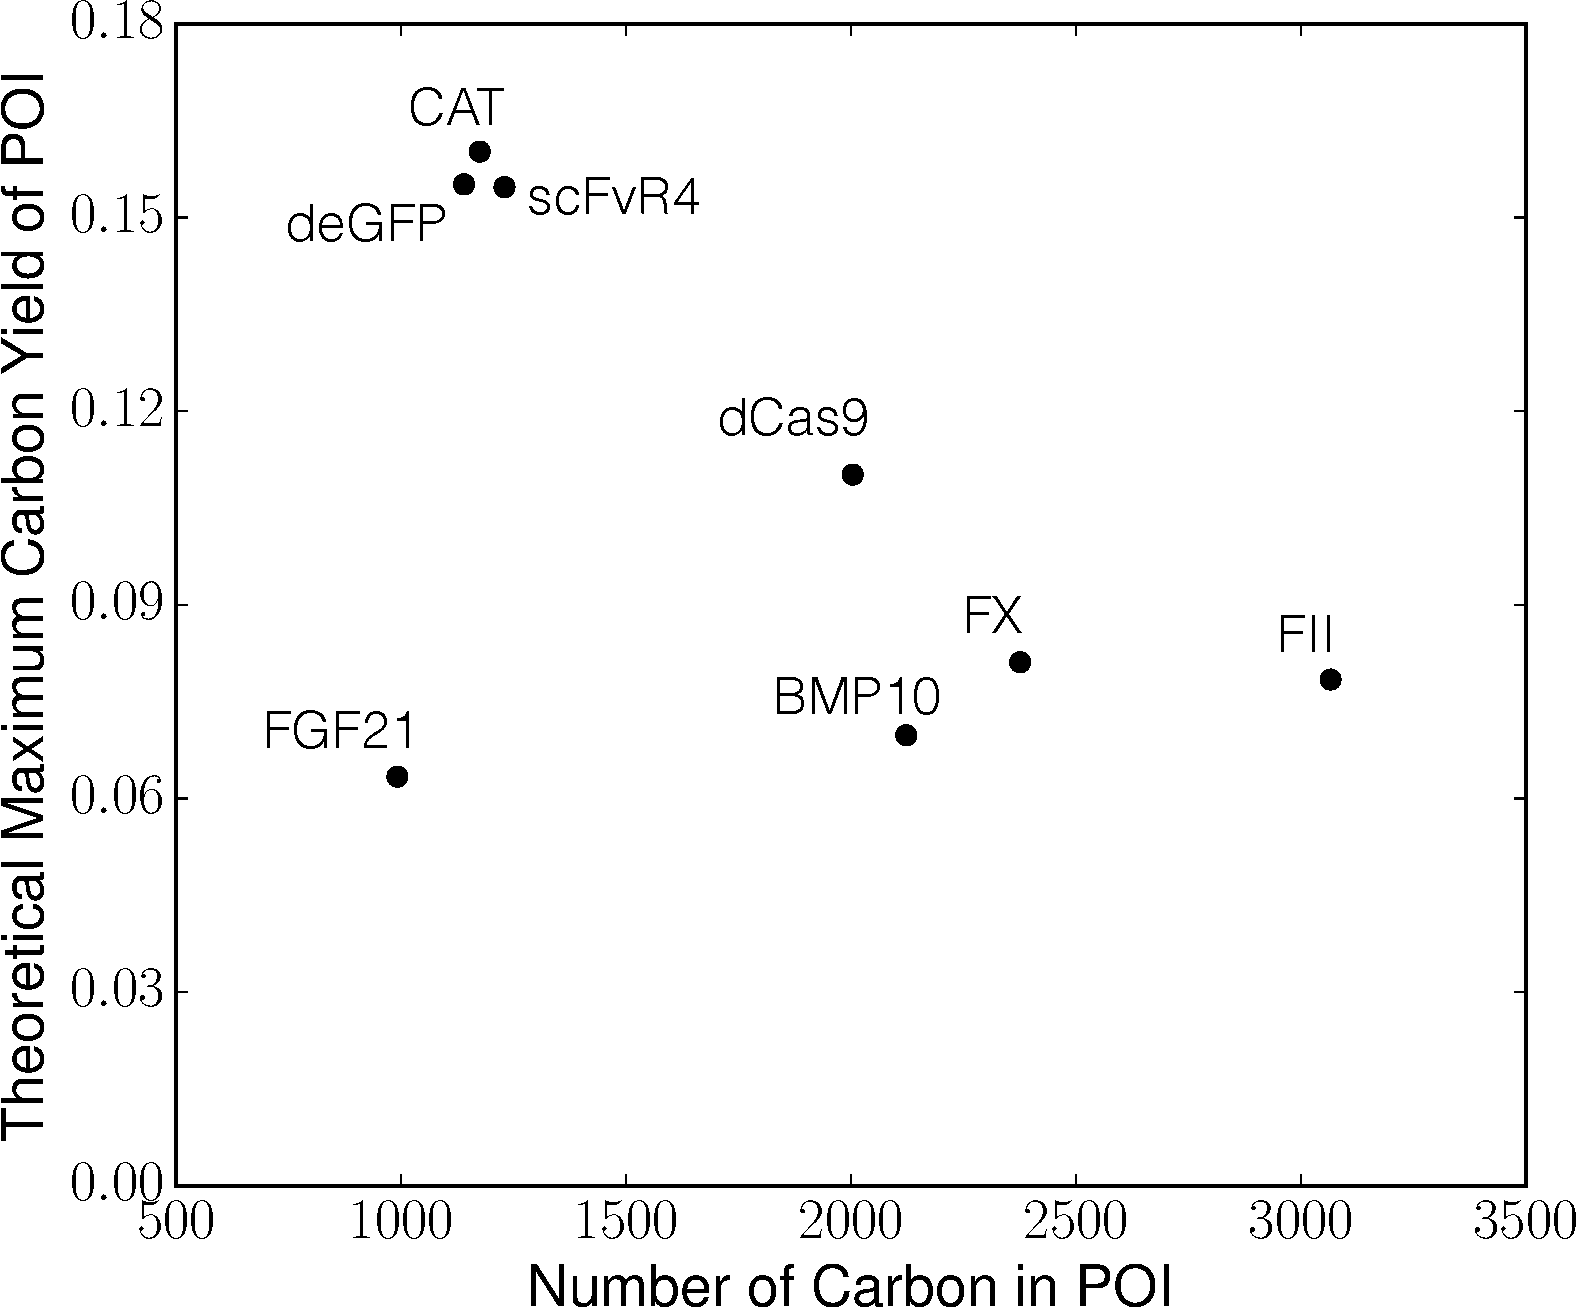
\includegraphics[width=0.45\textwidth]{./figures/YieldNumber.pdf}
\caption{Theoretical maximum carbon yield of nine proteins versus the corresponding carbon number of each protein. There is a relative inverse relationship of carbon yield to number of carbons in each protein except for the protein FGF21. 
}
\label{fig:YieldNumber}
\end{figure}




\clearpage
\section*{Discussion}

\clearpage

\section*{Materials and Methods}

\subsection*{Formulation and solution of the model equations.}
The flux balance analysis problem was formulated as:
\begin{equation}\nonumber
 \begin{multlined}
	\qquad \qquad \qquad \max_{\boldsymbol{w}}{} \! \left( w_{obj} = \mathbf{\boldsymbol{\theta}}^T \boldsymbol{w} \right) \\
	\mathrm{Subject \; to:}
	 \; \; \mathbf{S}\mathbf{w}=\mathbf{0} \\
\alpha_i \leq w_i \leq \beta_i  \qquad i=1,2,\hdots,\mathcal{R}
 \end{multlined}
\end{equation}
where $\mathbf{S}$ denotes the stoichiometric matrix, $\mathbf{w}$ denotes the unknown flux vector, $\boldsymbol{\theta}$ denotes the objective selection vector
and $\alpha_i$ and $\beta_i$ denote the lower and upper bounds on flux $w_{i}$, respectively.
The flux balance analysis problem was solved using the GNU Linear Programming Kit (v4.52) \cite{GLPK}.
In this study, the objective $w_{obj}$ was to maximize the production of circuit output.
The specific glucose uptake rate was constrained to allow a maximum flux of 10 mmol/hr \cite{2002_Mahadevan_BiophysJ}; the amino acids were also bound to allow a maximum flux of 10 mmol/hr, but did not reach this maximum flux.

\subsection*{Transcription and translation template reactions.}
The transcription and translation template reactions are based off sequence specific FBA \cite{2002_allen_palsson} involving transcription initiaion, transcription, mRNA degradation, translation initiation, translation, and tRNA charging. 
The mRNA and protein sequence of each protein was determined from literature. 
The transcription rate was constrained by the following formulation:

\begin{equation}\nonumber
	w_{tx} = [RNAP]\frac{v_{RNAP}}{l_{mRNA}}\left(\frac{[Gene]}{km+[Gene]}\right)P
\end{equation}

where $[RNAP]$ is the concentration of RNA polymerase which was determined from literature values based on the number of copies per cell, $v_{RNAP}$ is the elongation rate (nucleotides/hr) of the RNA polymerase, $l_{mRNA}$ is the number of nucleotides in the mRNA for the protein of interest, $[Gene]$ is the gene concentration of the protein of interest, $km$ is the plasmid saturation coefficient, and $P$ is the promoter activity. 
The promoter activity was formulated following Moon et al. for synthetic circuits by the following:

\begin{equation}\nonumber
	P = \frac{K_{1}+K_{2}f_{p70}}{1 + K_{1}+K_{2}f_{p70}}
\end{equation}

where $K_{1}$ represents the state of RNA polymerase binding, $K_{2}$ is the state of sigma-70 binding along with RNA polymerase, and $f_{p70}$ is the fraction of the transcription factor, sigma-70, bound to the promoter following Hills kinetics. 

The translation rate was constrained by the following formulation:

 \begin{equation}\nonumber
	w_{tl} = [Ribo]K_{P}\frac{v_{Ribo}}{l_{protein}}[mRNA_{ss}]
\end{equation}

where $[Ribo]$ is the ribosome concentration determined from literature values based on the number of copies per cell, $K_{P}$ is the polysome amplification constant, $v_{Ribo}$ is the elongation rate (amino acids/hr) of the ribosome, $l_{protein}$ is the number of amino acids in the protein of interest, and $[mRNA_{ss}]$ is the mRNA concentration at steady state determined by the transcription rate divided by the degradation rate of mRNA.  

\subsection*{Theoritical carbon yield.}
The theortical carbon yield of each protein was formulated as:

\begin{equation}\nonumber
	Yield = \frac{C_{POI}v_{POI}}{\sum_{i = 1}^{\mathcal{R}}C_{i}v_{i}}
\end{equation}

where $C_{POI}$ and $C_{i}$ denote the carbon number of the protein of interest (POI) and substrate $i$, respectively, $v_{POI}$ and $v_{i}$ denote the flux of the POI and substrate $i$, respectively,
and $\mathcal{R}$ denotes the number of substrates consumed.


\subsection*{Global sensitivity analysis.}
We conducted a global sensitivity analysis, using the variance-based method of Sobol, to estimate which parameters controlled the performance of synthetic circuits \citep{SOBOL_METHOD}.
We computed the total sensitivity index of each parameter relative to two performance objectives, the peak thrombin time and the area under the thrombin curve (thrombin exposure).
We established the sampling bounds for each parameter from the minimum and maximum value of that parameter in the parameter set ensemble.
We used the sampling method of Saltelli \textit{et al.} \citep{Saltelli:2010} to compute a family of $N\left(2d+2\right)$ parameter sets which obeyed our parameter ranges,
where $N$ was the number of trials, and $d$ was the number of parameters in the model. In our case, $N$ = 10,000 and $d$ = 22, so the total sensitivity indices were computed from
460,000 model evaluations. The variance-based sensitivity analysis was conducted using the SALib module encoded in the Python programming language \citep{SALIB}.

\clearpage

\section*{Acknowledgements}
This study was supported by an award from the Army Research Office (ARO \#59155-LS).
\clearpage

\bibliography{References_v1}

\clearpage

% Supplemental figures -
% Set the S-
\renewcommand\thefigure{S\arabic{figure}}
\renewcommand\thetable{T\arabic{table}}
\renewcommand\thepage{S-\arabic{page}}
\renewcommand\theequation{S\arabic{equation}}

% Reset the counters -
\setcounter{equation}{0}
\setcounter{table}{0}
\setcounter{figure}{0}
\setcounter{page}{1}

\end{document}
